% !TeX root = ../main.tex
\begin{figure}[htbp]
  \centering
  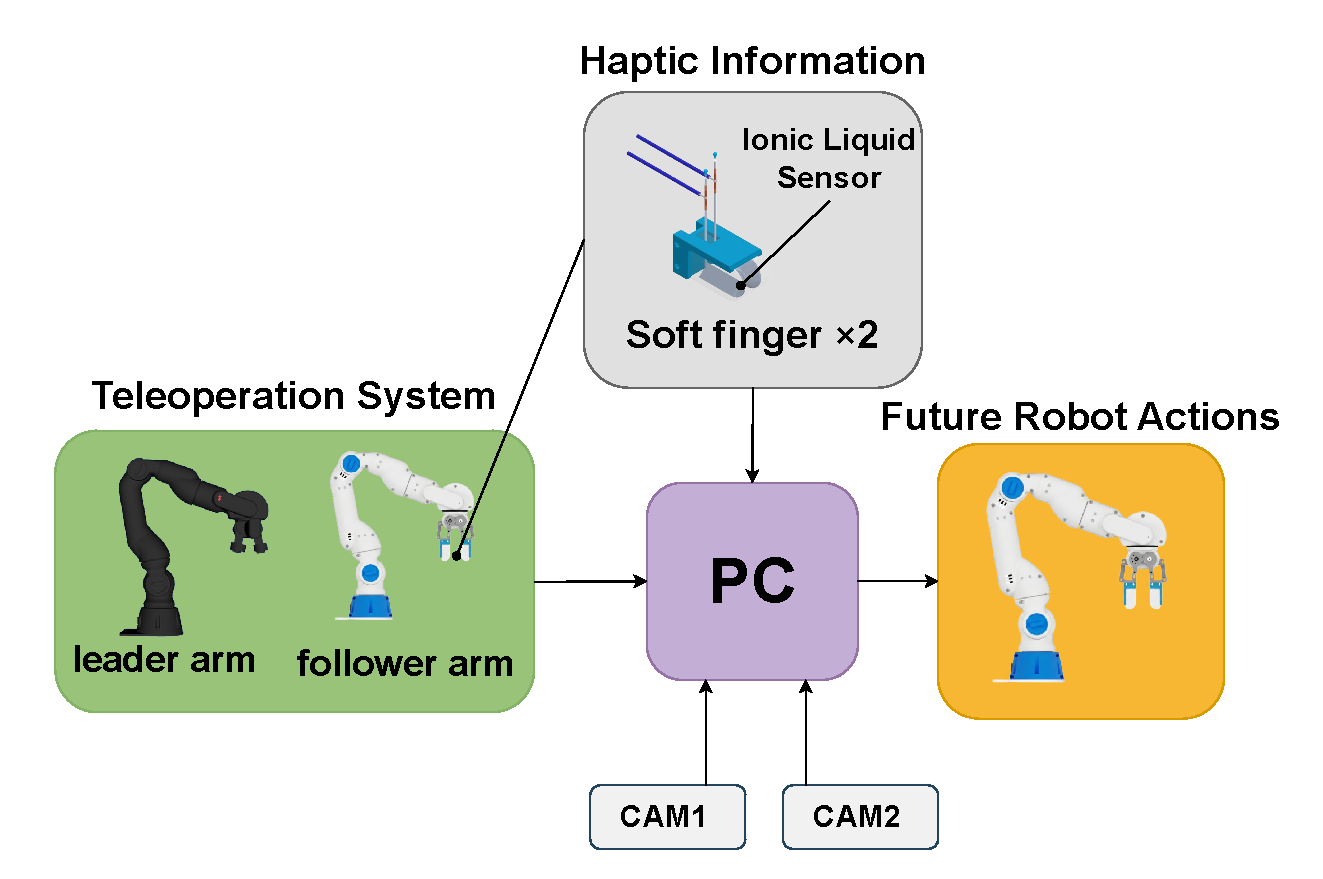
\includegraphics[width=0.95\linewidth]{tex/Image/imitationlearningsystemrobomech.drawio.pdf}
  \caption{Overview of the proposed imitation learning system using a teleoperation setup and haptic information}
  \label{fig:robot_system}
\end{figure}
% 本章では，提案する模倣学習手法について述べる．Fig\ref{fig:robot_system}にシステムの構成図を示す．
本システムは，リーダー・フォロワー構成のロボットアーム，フォロワーアーム先端に2つのイオン液体センサを内蔵したソフトフィンガー，フォロワーアームを側面・上面から観測するRGBカメラ2台，および制御・学習用PCで構成される．教示データ収集時は操作者がリーダーアームを操作し，フォロワーアームで物体操作を行う．収集データを用いてフォロワーアームの動作モデルを模倣学習し，入力にはカメラ画像，関節角度，ソフトフィンガーの触覚情報を用いる．学習後は，フォロワーアームが自律的に物体操作タスクを実行する．\par

まず，ハードウェア構成を述べる．本研究では，リーダー・フォロワー方式のテレオペレーションシステムとして，RT社製7自由度ロボットアームCRANE-X7を2台使用する．アーム7自由度とグリッパ1自由度を備え，全体で8自由度である．1台をリーダー，もう1台をフォロワーとして用い，フォロワーのグリッパにソフトフィンガーを取り付けている．\par
このフィンガーはシリコンゴム本体とPLA製の爪部からなり，内部にイオン液体を封入した流路を持つ触覚センサを埋め込んでいる．イオン液体は導電性に加え，不揮発性，難燃性，高い熱安定性を有する\cite{armandIonicliquidMaterialsElectrochemical2009}．対象物との接触で流路が変形すると，断面積 $A$ と長さ $L$ が変化する．
この幾何学的変化は，イオン液体固有の電気抵抗率 $\rho$ を用いて，抵抗値 $R$ が次式
\begin{equation}
  R = \rho \frac{L}{A}
\end{equation}
で表されるため，検出できる\cite{chossatSoftStrainSensor2013}．フォロワーアームには平行リンク機構を用いた2指平行グリッパを取り付け，2つのソフトフィンガーからセンサ情報を取得する．\par
% \begin{figure}[htbp]
%   \centering
%   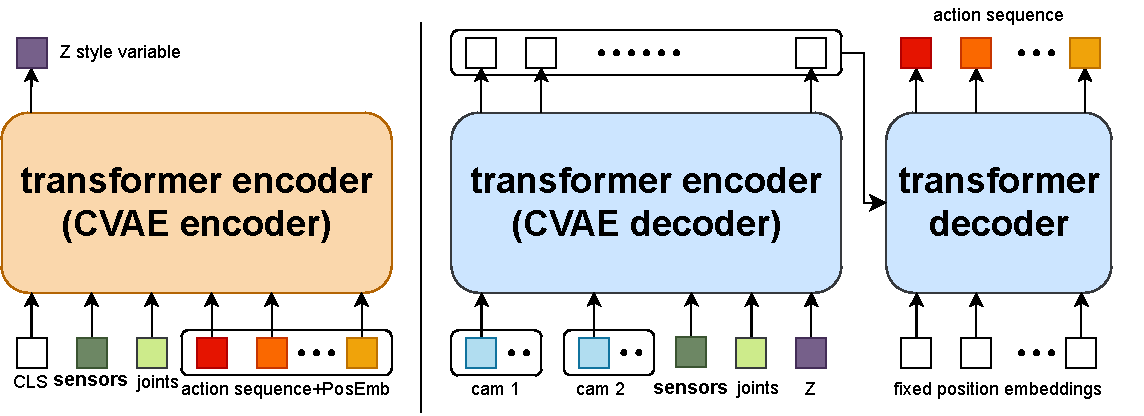
\includegraphics[width=1.1\linewidth]{tex/Image/ACT.drawio.pdf}
%   \caption{Action Chunking with Transformers (ACT) architecture used for imitation learning．This model extends the conventional ACT framework by introducing distinct sensor embeddings．}
%   \label{fig:act}
% \end{figure}
本研究では，接触を伴う複雑タスクを7自由度ロボットアームで学習するため，Action Chunking with Transformers (ACT) \cite{zhaoLearningFineGrainedBimanual2023}を採用する．ACTはConditional Variational Autoencoder (CVAE)とTransformerを組み合わせたモデルで，現在の観測から未来数ステップのアクション系列（Action Chunk）を一括予測することで，時系列の長期依存を学習し，滑らかな動作生成を実現する．本アーキテクチャの特徴は，従来のACTにセンサ値を新たなモダリティとして追加した点である．関節角度と同様にセンサ値をトークン化し，CVAEエンコーダーとデコーダーに画像特徴量・関節情報と並列入力することで，触覚を統合した動作生成を可能にした．実装には，Hugging Faceが提供する模倣学習ライブラリlerobot\cite{cadene2024lerobot}を用いた．\par
リーダーアーム操作時は，CRANE-X7の重量負担を軽減するため重力補償制御を適用する．現在の関節位置から各関節に作用する重力トルクを計算し，逆方向のトルクを各関節に加えてアーム重量を相殺することで，操作者は質量感を抑えた直感的な教示動作を行える．
% lerobotはデータ収集から学習，評価までを統一的に扱える優れたフレームワークであるが，重力補償機能はPython実装では制御周期の安定性やリアルタイム性に課題があった．そこで本研究では，RT社の提供するCRANE-X7の重力補償のC++ライブラリをpybind11を用いてlerobotのPython環境に組み込む実装を行った．これにより，最新の学習フレームワークの恩恵を受けつつ，C++による滑らかで高応答な重力補償制御を両立させている．